\documentclass[10pt,a4paper]{article}
\usepackage[utf8]{inputenc}
\usepackage[a4paper]{geometry}
\usepackage{amsmath}
\usepackage{stmaryrd}
\usepackage{fullpage}
\usepackage{multicol}
\usepackage[usenames,dvipsnames]{color}
\usepackage{graphicx}
%\usepackage[landscape]{geometry}
%needs to be defined before using the pdftex package
\definecolor{linkcolor}{rgb}{0.1,0.0,0.35}
\definecolor{citecolor}{rgb}{0.1,0.0,0.35}
\definecolor{unchangedcolor}{rgb}{0.4,0.4,0.4}
%\definecolor{unchangedcolor}{rgb}{0.2,0.2,0.6}
\definecolor{changedcolor}{rgb}{1.0,0.2,0.0}
\usepackage[pdftex,
            colorlinks=true,
            linkcolor=linkcolor,
            filecolor=red,
            citecolor=citecolor,
            pdftitle={TLAPM v2 Architecture},
            pdfauthor={Martin Riener},
            pdfsubject={},
            pdfkeywords={},
            bookmarks, bookmarksnumbered=true]{hyperref}
\usepackage{cite}
\usepackage{url}

\usepackage{todonotes}
\definecolor{todocolor}{rgb}{0.9,0.5,0.5}
\newcommand{\itodo}[1]{\todo[inline]{TODO: #1}}
\newcommand{\iremark}[1]{\todo[inline]{REMARK: #1}}
\newcommand{\question}[1]{\todo[inline, color=blue!35]{QUESTION: #1}}
\newcommand{\problem}[1]{\todo[inline, color=red!35!blue!35!white]{PROBLEM: #1}}
\newcommand{\todofootnote}[1]{{\todo{TODO: #1}}}
\newcommand{\questionfootnote}[1]{{\todo[color=blue!35]{QUESTION: #1}}}
\newcommand{\problemfootnote}[1]{\todo[color=red!35!blue!35!white]{PROBLEM: #1}}

\newcommand{\commentout}[1]{ }


\newcommand{\sub}[2]{\ensuremath{#1 \mapsfrom #2 }}
\newcommand{\subst}[1]{\ensuremath{\{#1\}}}
\newcommand{\filename}[1]{\texttt{#1}}
\newcommand{\modulename}[1]{\texttt{#1}}
\newcommand{\datatype}[1]{\texttt{#1}}
\newcommand{\keyword}[1]{\textsc{#1}}

\newcommand{\dtlambda}{\datatype{lambda}}
\newcommand{\dtuop}{\datatype{user\_defined\_op}}
\newcommand{\dtopdef}{\datatype{op\_def}}
\newcommand{\dtopdecl}{\datatype{op\_decl}}
\newcommand{\dtdefinedexp}{\datatype{defined\_expr}}
\newcommand{\dtopappl}{\datatype{op\_appl}}
\newcommand{\dtsubst}{\datatype{subst\_in}}
\newcommand{\dtapsubst}{\datatype{ap\_subst\_in}}
\newcommand{\dtexpr}{\datatype{expr}}
\newcommand{\dtap}{\datatype{assume\_prove}}



\title{TLAPM v2 Architecture}

\begin{document}
\maketitle

\section{Introduction}
\label{sec:introduction}
The TLA Proof Manager (PM) reads a TLA+ specification and extracts the
 expressions needed to prove the steps of its theorems. These expressions are
 called proof obligations. A backend convert an obligation into suitable
 input for a theorem prover. At the moment, there exist backends for
 Isabelle/TLA, Zenon, SMT and LS4 where each of them covers a different subset
 of the language.

The rewrite of the PM adresses the following problems:

\begin{itemize}
\item Properties about \keyword{ENABLED} can only be proved by coalescing (which
 is incomplete)
\item Temporal quantifiers don't have backend
\item Recursively defined operators are not expanded
\item The data-structures of the current PM are mutable and have deBruijn
 indices, making debugging exceptionally complicated
\item The languages accepted by toolbox and the PM need to agree. In case of
 conflicting interpretations, the language accepted by the toolbox is
 authoritative. The easiest way to prevent disagreement is to share the parser
 between the toolbox and the PM.
\end{itemize}


\section{General Architecture}
\label{sec:general}

SANY, the abstract syntax tree used in the toolbox, is implemented in Java,
 wheras the PM is implemented in OCaml. The first step is to serialze the Java
 datastructures to XML and recreate them in OCaml (see section \ref{sec:sany}).
 Since the SANY datastructures are considered as static, the second step
 converts them to the internal syntax tree (see section \ref{sec:exprds}).
 After applying some processing steps, the specification is divided into
 a list of obligations. The backends (section \ref{sec:backends}) are resposible
 for exporting an obligation to a theorem prover and the quering of the results.
 The status of each obligation proof attempt is communicated back to the Toolbox
 via standard output using a text-based protocol (section \ref{sec:protocol}).

 \begin{figure}[htb]
   \centering
   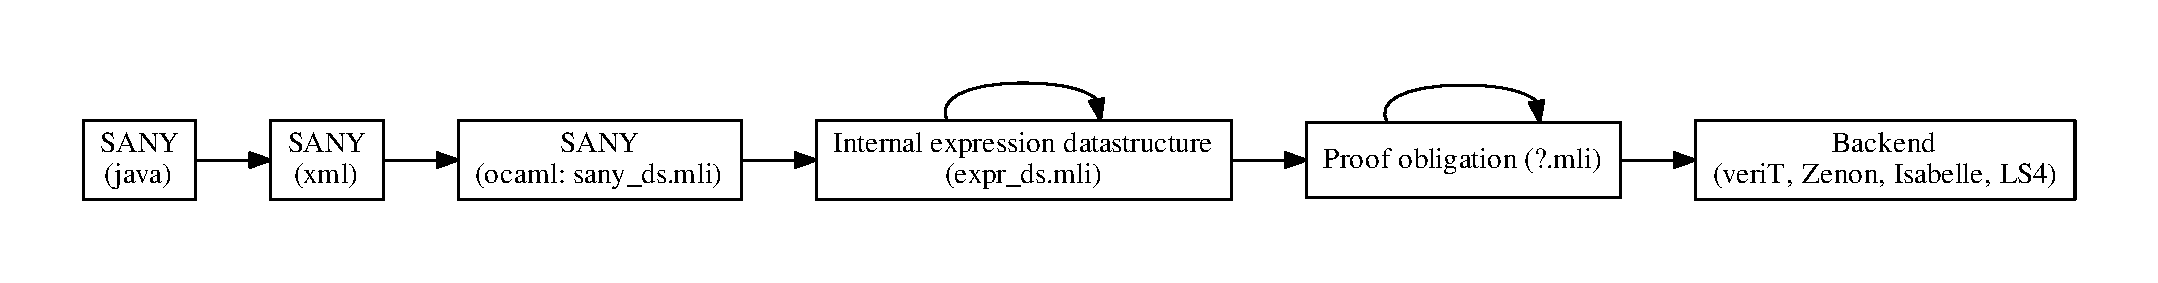
\includegraphics[width=\textwidth]{architecture.pdf}
   \caption{Architecture Overview - Data Structures}
   \label{fig:datastructures}
 \end{figure}
\section{SANY Import (sany\_*.mli)}
\label{sec:sany}
\itodo{explain more about the naming structure, containment etc}

\section{Internal Datastructure (expr\_*.mli)}
\itodo{explain more about the naming structure, containment etc}

All of these are universal for the whole spec:
\label{sec:exprds}
\begin{itemize}
\item Resolve explicit substitutions
 (Problem: does not distribute over ENABLED?)
\item $\beta$-reduce lambda expressions
\item $\lambda$-abstraction is realized as application. replace by explicit
 lambda operator (an expression).
\item replace @ notation by the expressions they stand for
\item replace ! notation by what it refers to
\item  let-in?
\item remove theorems from submodules, replace named theorems by user-defined
 operators
\end{itemize}


\subsection{The Difference between Instantiation and Substitution}
\label{sec:instantiation-difference}
\itodo{Substitutions occur when unfolding definitions and applications of
 $\lambda$-abstractions. Instantiation replaces operator declarations by
 expressions. Substiutions recurse into \keyword{ENABLED}, but instantiation
 needs to unfold \keyword{ENABLED}.
}




\subsection{Changing the application workaround to $\lambda$-abstractions}
\label{sec:lambda}

The SANY parser does not have its own data-structure for $\lambda$-abstractions.
 Instead, for the expression $\lambda x:expr$ a dummy definition
 $\keyword{LAMBDA}(x) == expr$ is introduced, which is then applied
\footnote{Since there is no partial evaluation in TLA+, it is always applied to
 the all the formal parameters abstracted over.}. This is safe, because
 \keyword{LAMBDA} is a reserved word of the language and therefore not allowed
 as a definition name.
 In some cases\footnote{e.g. \filename{test/resources/tla/minilambda.tla}}, the
 construct created introduces a second dummy operator $O$: there, the
 substitution \subst{\sub{O}{ \lambda x, y : expr}} is applied to the expression
 $O(x, y)$.

The module \modulename{Expr\_correct\_lambda}\footnote{
\filename{src/expr\_correct\_lambda.ml}} contains an algorithm
 which replaces the \keyword{LAMBDA} definitions by \dtlambda{}
 data-structures.
 What is problematic is that an \dtuop can occur in places
 where a \dtlambda{} is not allowed, even when it is wrapped into an
 \dtexpr{}. If we look at the type inclusion diagram (see
 appendix~\ref{app:lambda}), a \dtuop only occurs in form
 of an \dtopdef{} or a \dtdefinedexp{}. The latter is only used
 in proof datastructures, which do not refer to \keyword{LAMBDA} definitions
\footnote{This property is not checked at the moment.}.

 Moreover an \dtopdef{} occurs only as an
 \datatype{operator} argument in an \dtopappl{} or \datatype{at}
 expression or directly within a \datatype{let} expression. These are the
 patterns which actually need to be replaced. At the moment, only the
 \dtopappl{} case is handled though.

\subsection{Eliminating Explicit Substitution Operators}
\label{sec:substitution}
There are two explicit substitution operators in the internal data-structures:
 \dtsubst{} and \dtapsubst{}. Both contain a mapping from
 declared operators (\dtopdecl{}) to expressions (\dtexpr{}) with the only
 difference that the first applies to an \dtexpr{} and the second applies to an
 \dtap{}.

We encounter similar problems as in section~\ref{sec:lambda}, where an
 \dtexpr{} can not always inserted in place of a \dtopdecl{}.


\section{Obligations}
\label{sec:obligations}

The unfolding of definitions is the single transformation which depends on the
 proof context. Together with the list of declared operators, the ASSUME-PROVE
 statement of a theorem with unfolded definitions forms a proof obligation.

Since what is coalesced depends on the capabilities of the backend, it also
 applies to an obligation.

\section{Backends}
\label{sec:backends}

\section{Toolbox Protocol}
\label{sec:protocol}


\appendix

\section{Replacement patterns of \filename{expr\_correct\_lambda.ml}}
\label{app:lambda}
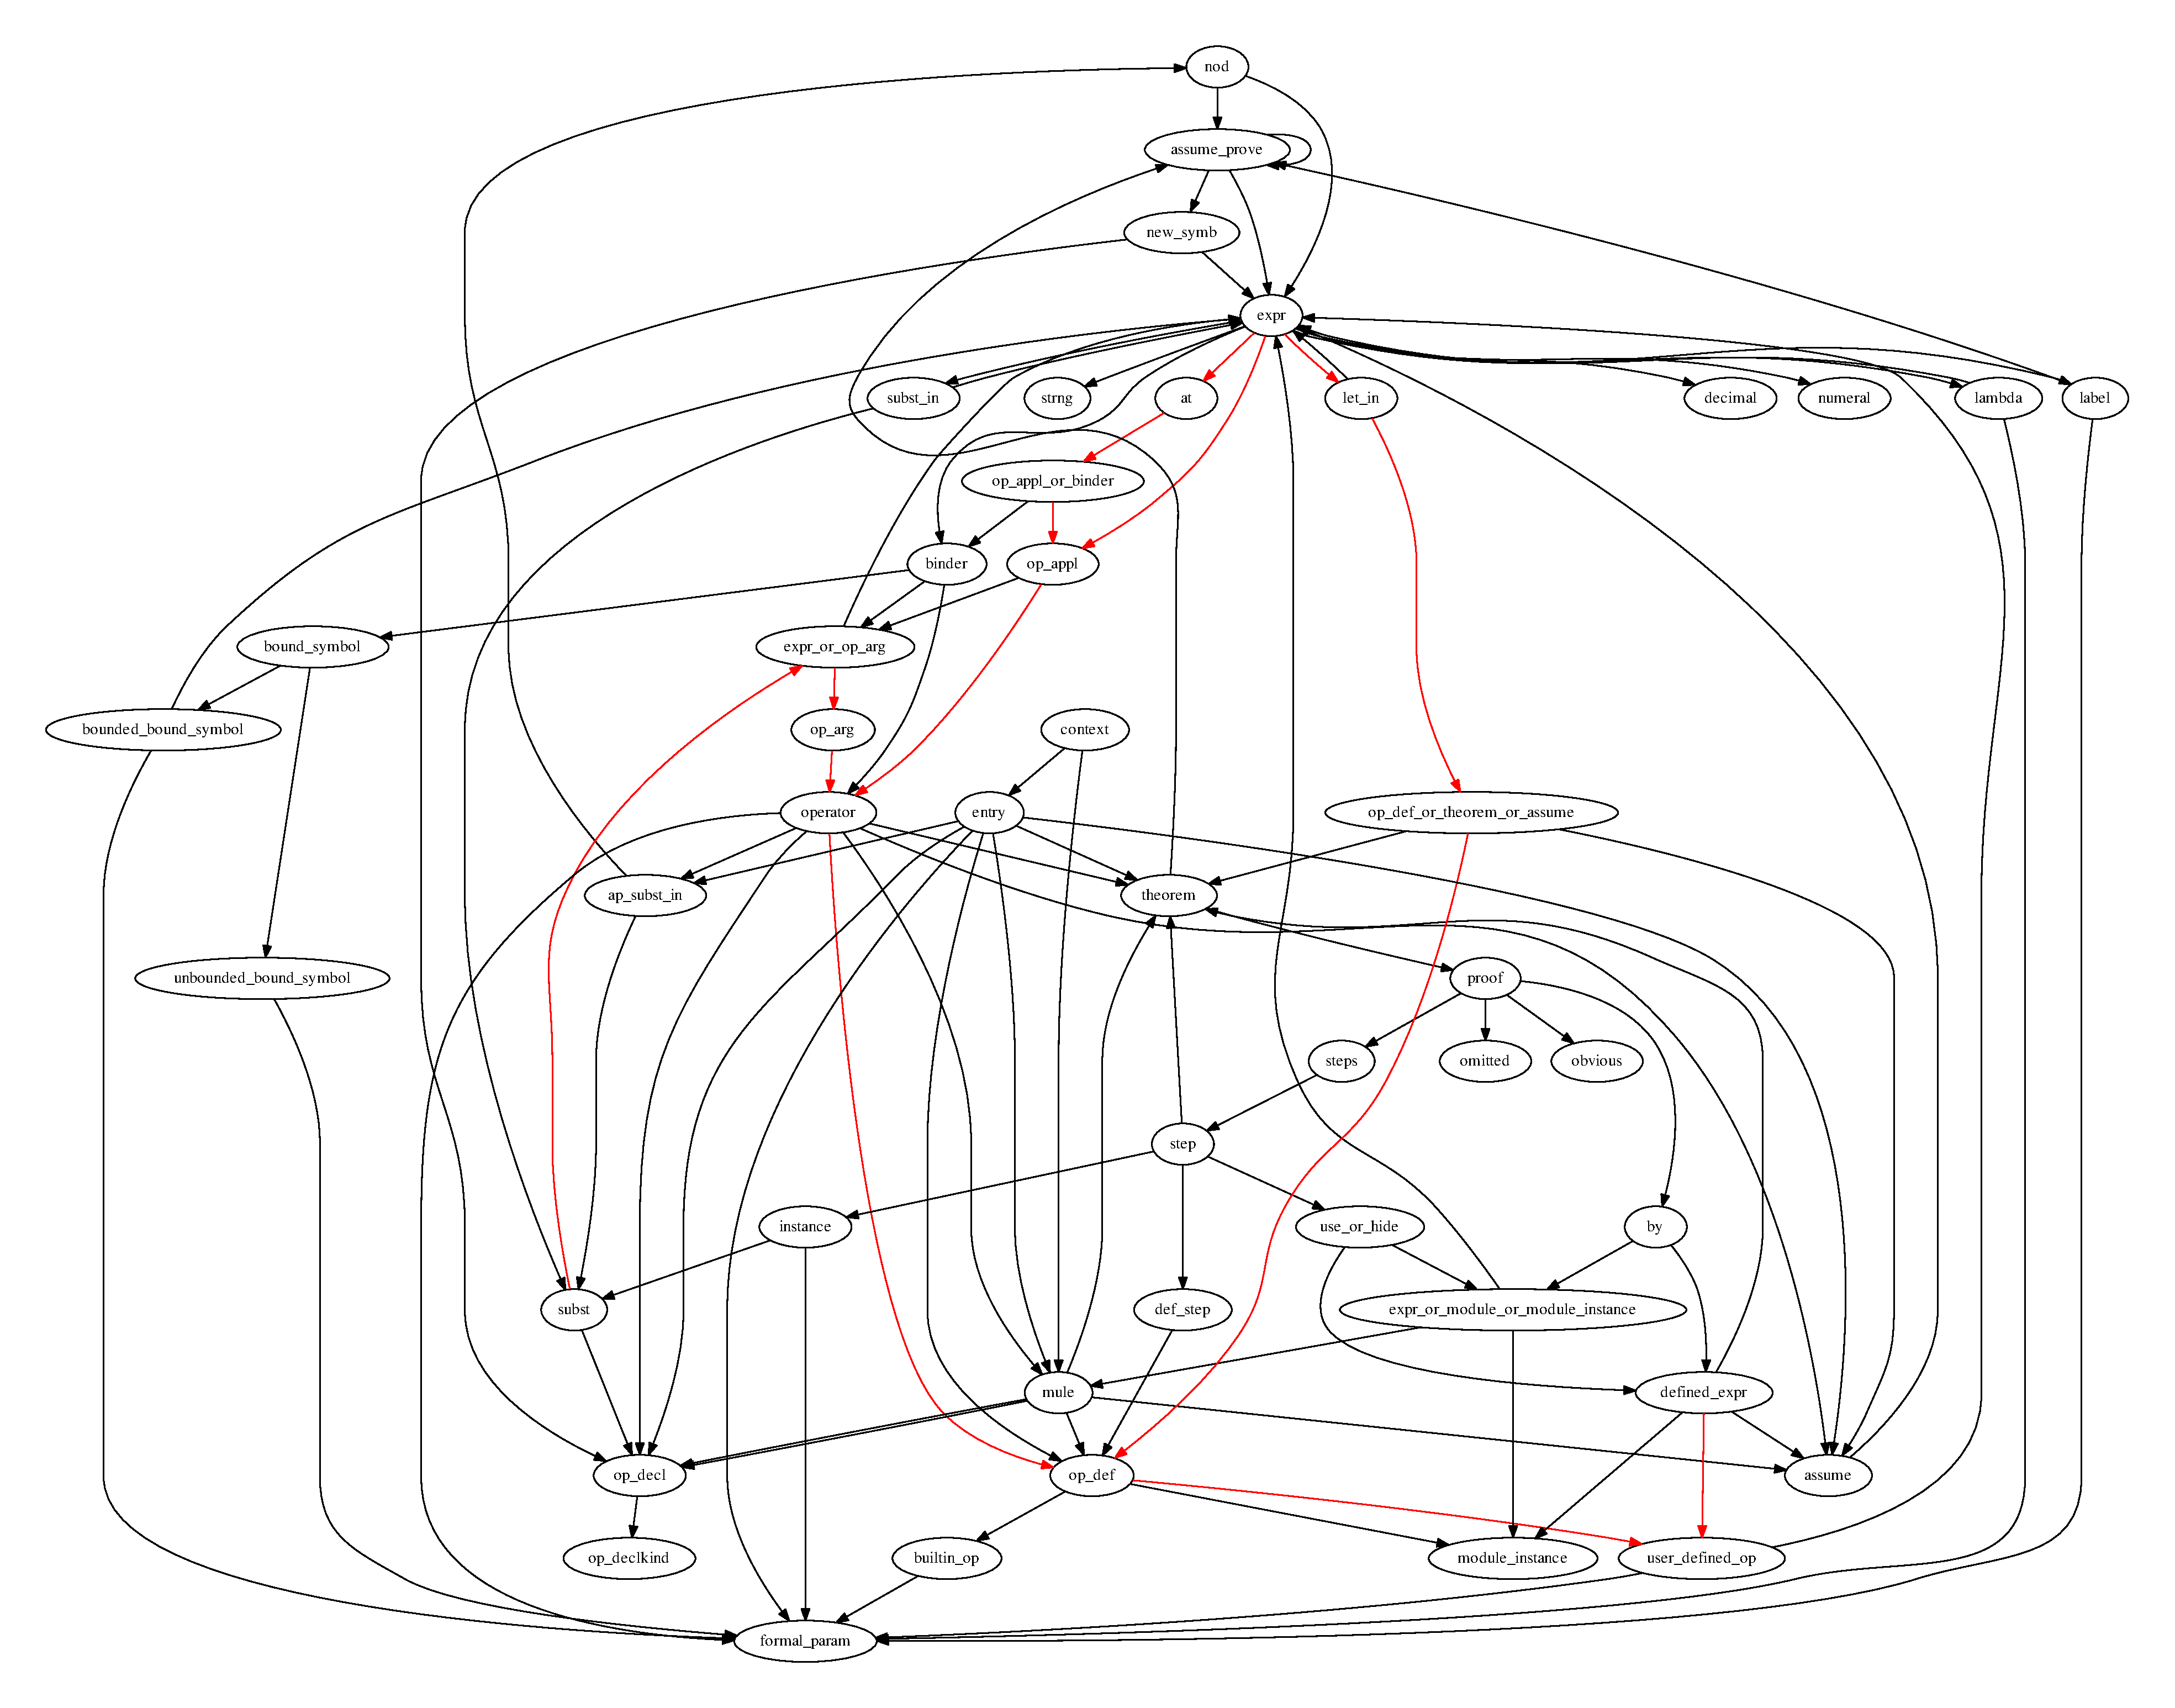
\includegraphics[angle=90,width=\textwidth]{lambda.pdf}

\section{Replacement patterns of \filename{?.ml}}
\label{app:lambda}
\includegraphics[angle=90,width=\textwidth]{subst.pdf}

\end{document}
